\section{(W) Static Obstacles and Constraints}\label{s:staticObstacles}
    \noindent Fast overview of obstacles and space constraints which position is static relative to mission time-frame:
    \begin{itemize}
        \item Static obstacles
        \item Geo-fencing areas (constraints)
        \item Long term bad weather areas (constraints)
		\item \emph{Constraint based path search} and \emph{obstacle modeling} is summarized in \cite{hentenryck2009constraint}.
    \end{itemize}
    \begin{figure}[H]
        \centering
        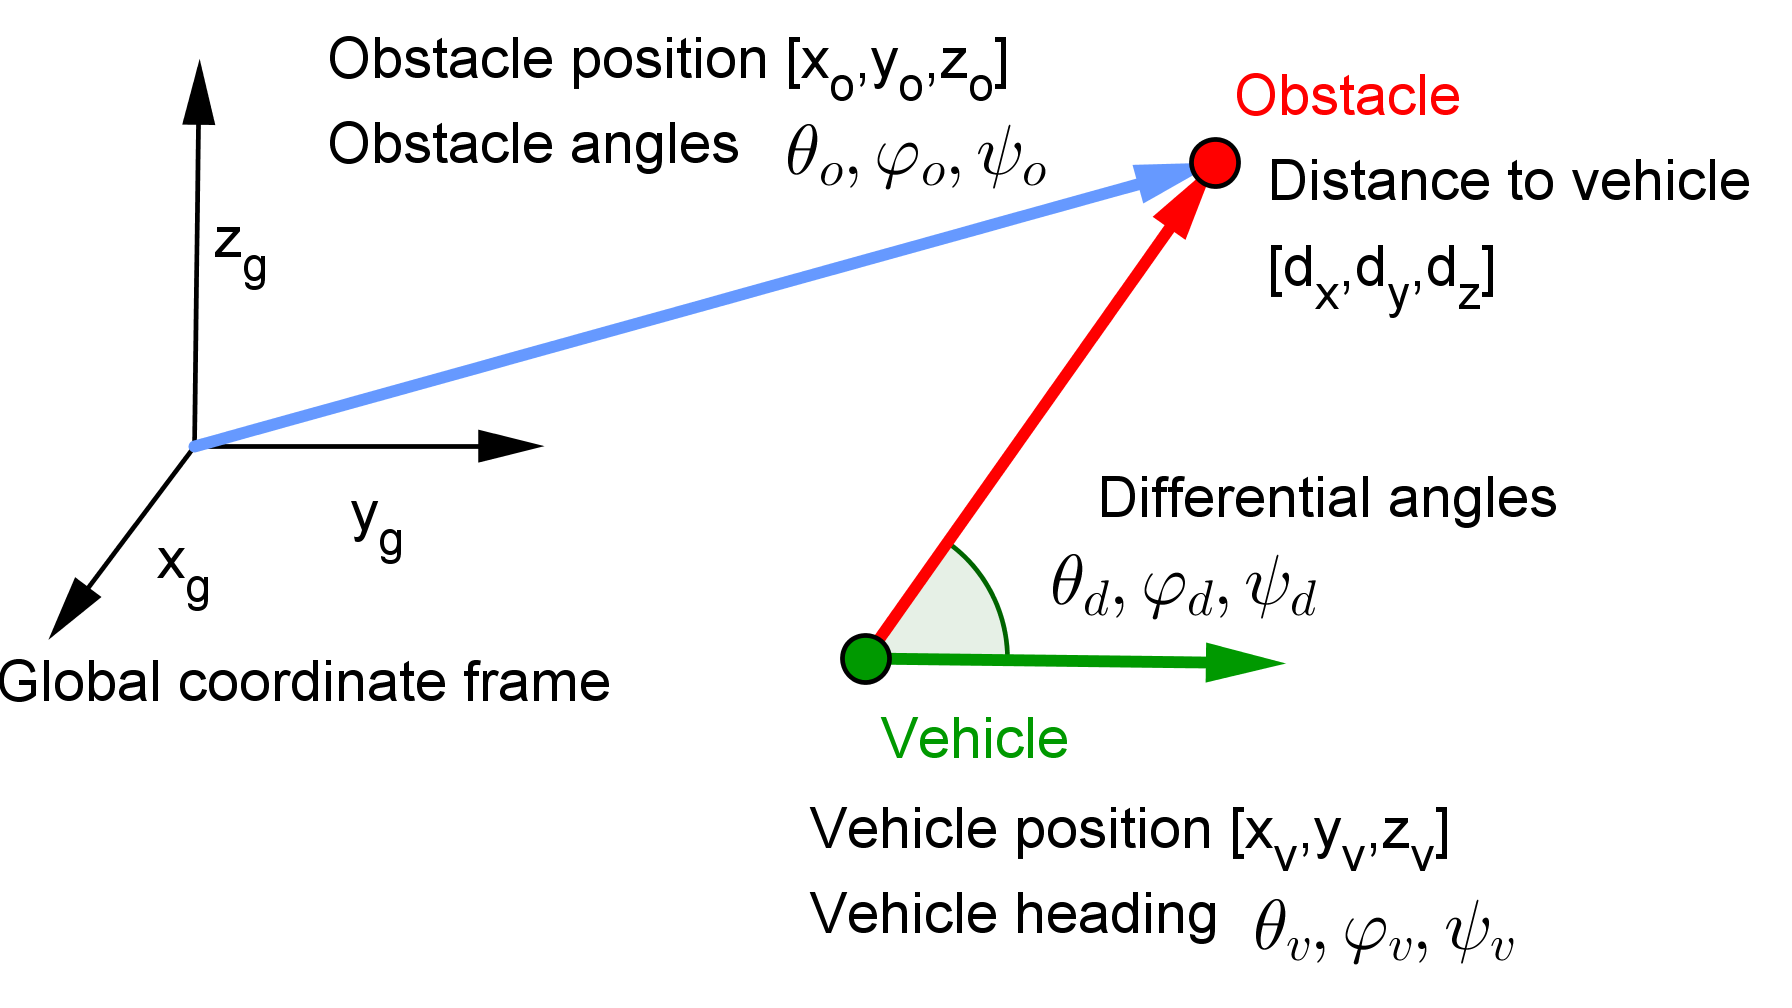
\includegraphics[width=0.6\linewidth]{\FIGDIR/TE022OsbtacleVehicleCoordinateFrameRelations} 
        \caption{Obstacle, UAS local, and UAS global coordinate frame relations.}
        \label{fig:coordinateFrameRelationsInFramework}
    \end{figure}
    
\subsection{(W) Detected obstacles}\label{s:detectedObstacles}
    \noindent Define certainty of obstacles (\emph{Sensor fusion}) (reuse some content from Linkoping work)

\subsection{(W) Map obstacles}\label{s:mapObstacles}
    \noindent Define certainty of obstacles from map (\emph{Data fusion}), (reuse some content from Linkoping work)
    \begin{figure}[H]
        \begin{subfigure}{0.32\textwidth}
            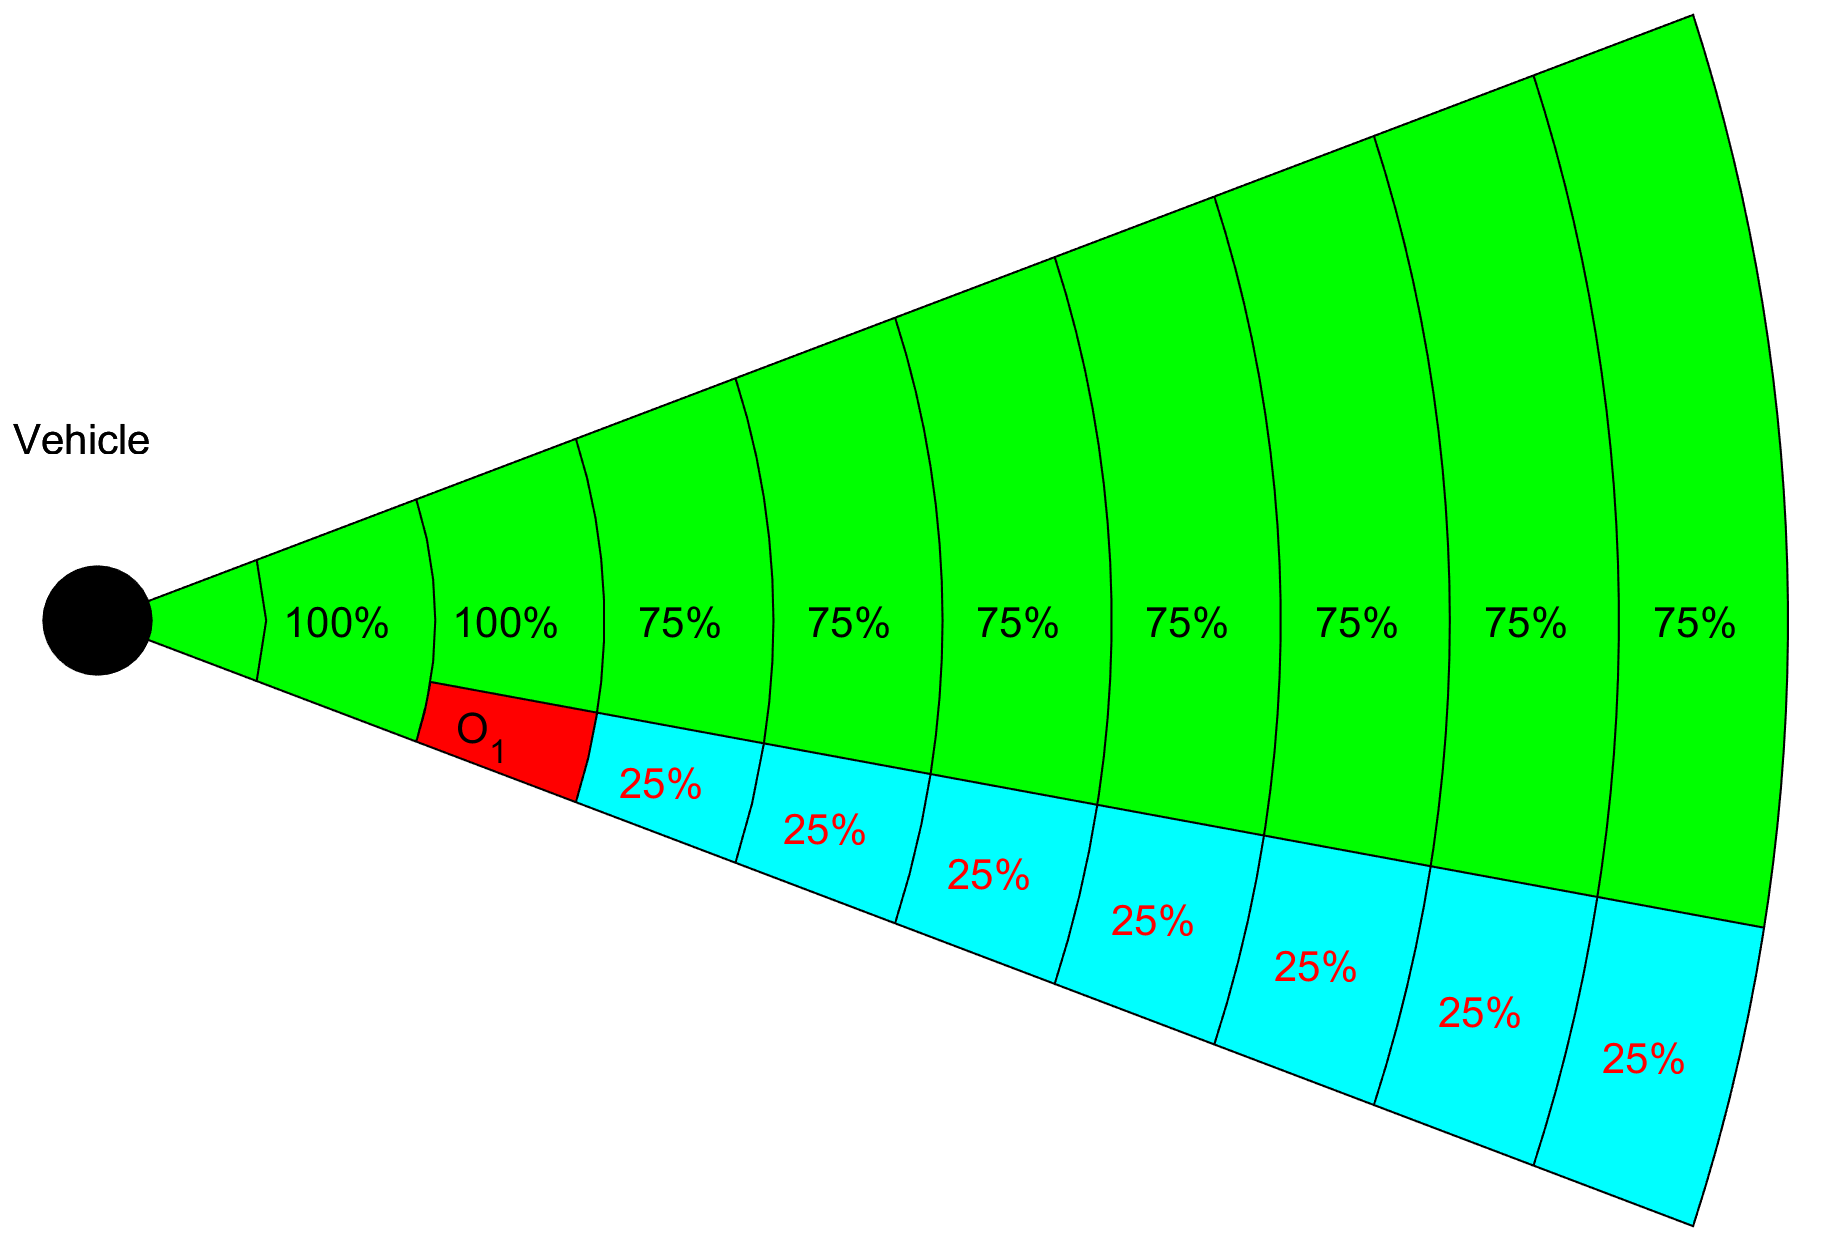
\includegraphics[width=0.9\linewidth]{\FIGDIR/TE006VisibilityFirstObstacle} 
            \caption{1\textsuperscript{st} hindrance.}
            \label{fig:fistObstacleHindrance}
        \end{subfigure}
        \begin{subfigure}{0.32\textwidth}
            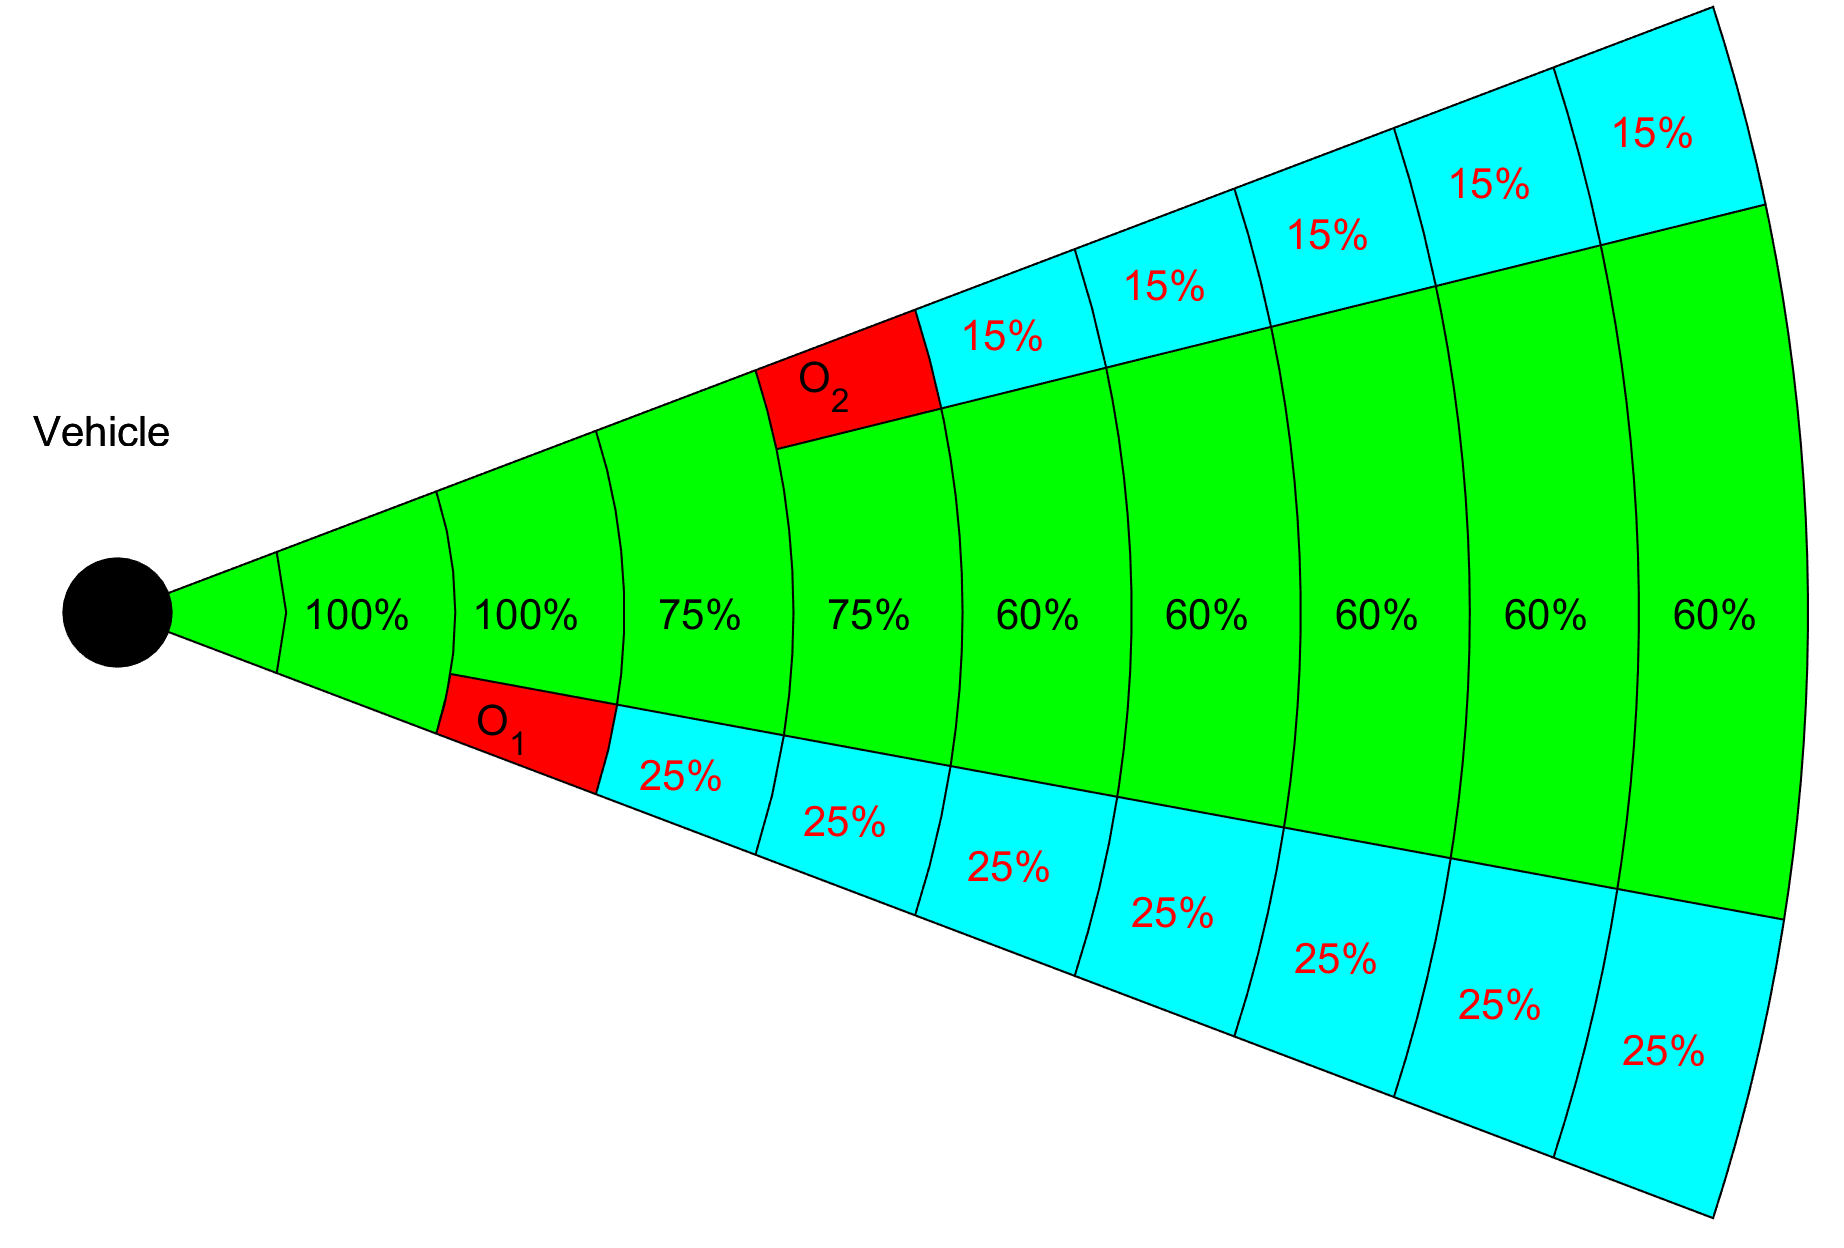
\includegraphics[width=0.9\linewidth]{\FIGDIR/TE007VisibilitySecondObstacle} 
            \caption{2\textsuperscript{nd} hindrance.}
            \label{fig:secondObstacleHindrance}
        \end{subfigure}
        \begin{subfigure}{0.32\textwidth}
            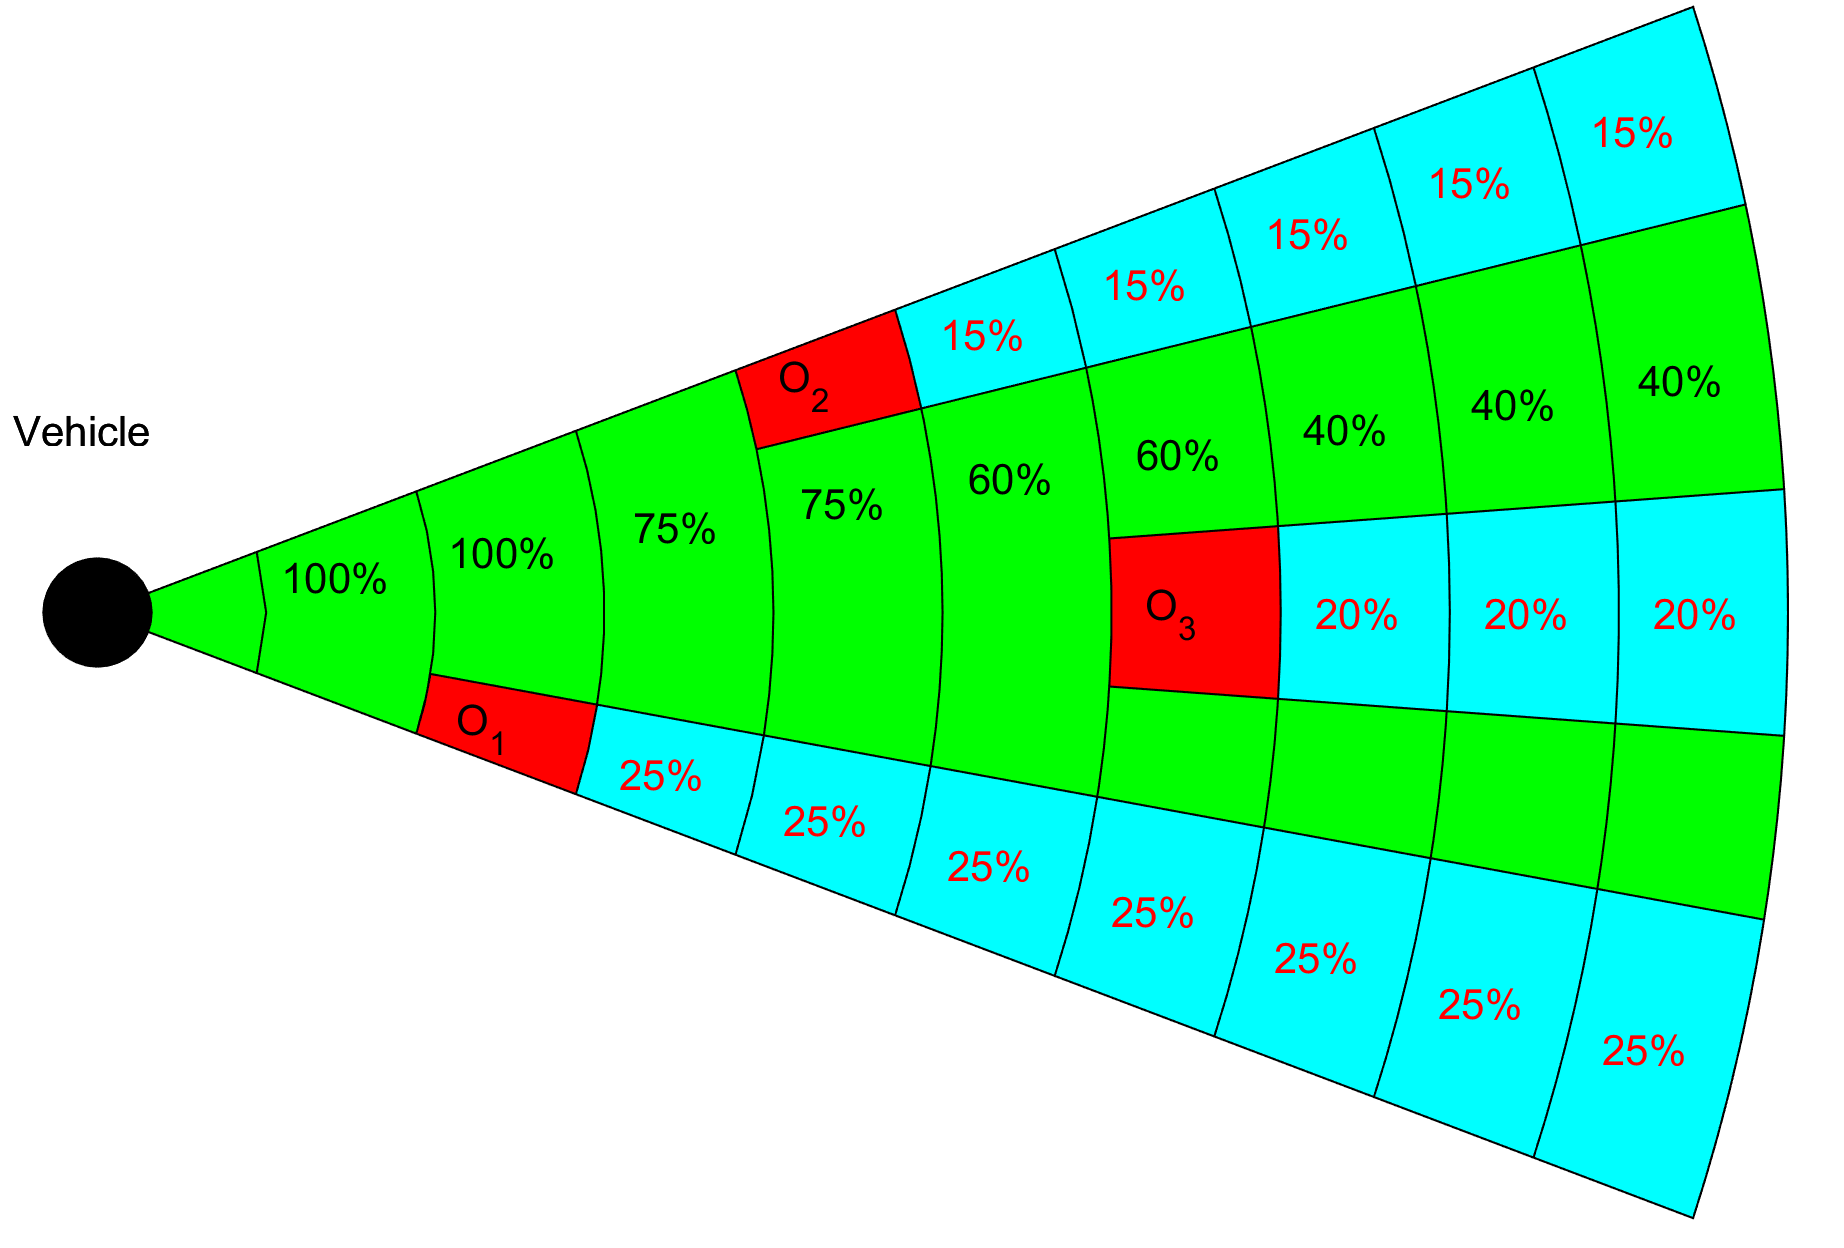
\includegraphics[width=0.9\linewidth]{\FIGDIR/TE008VisibilityThirdObstacle} 
            \caption{3\textsuperscript{rd} hindrance.}
            \label{fig:thirdObstacleHindrance}
        \end{subfigure}
        \caption{Obstacle hindrance impact on visibility in \emph{Avoidance Grid Slice}.}
        \label{fig:hindranceImpactOnVisibility}
    \end{figure}
    
    
    \begin{figure}[H]
        \begin{subfigure}{0.32\textwidth}
            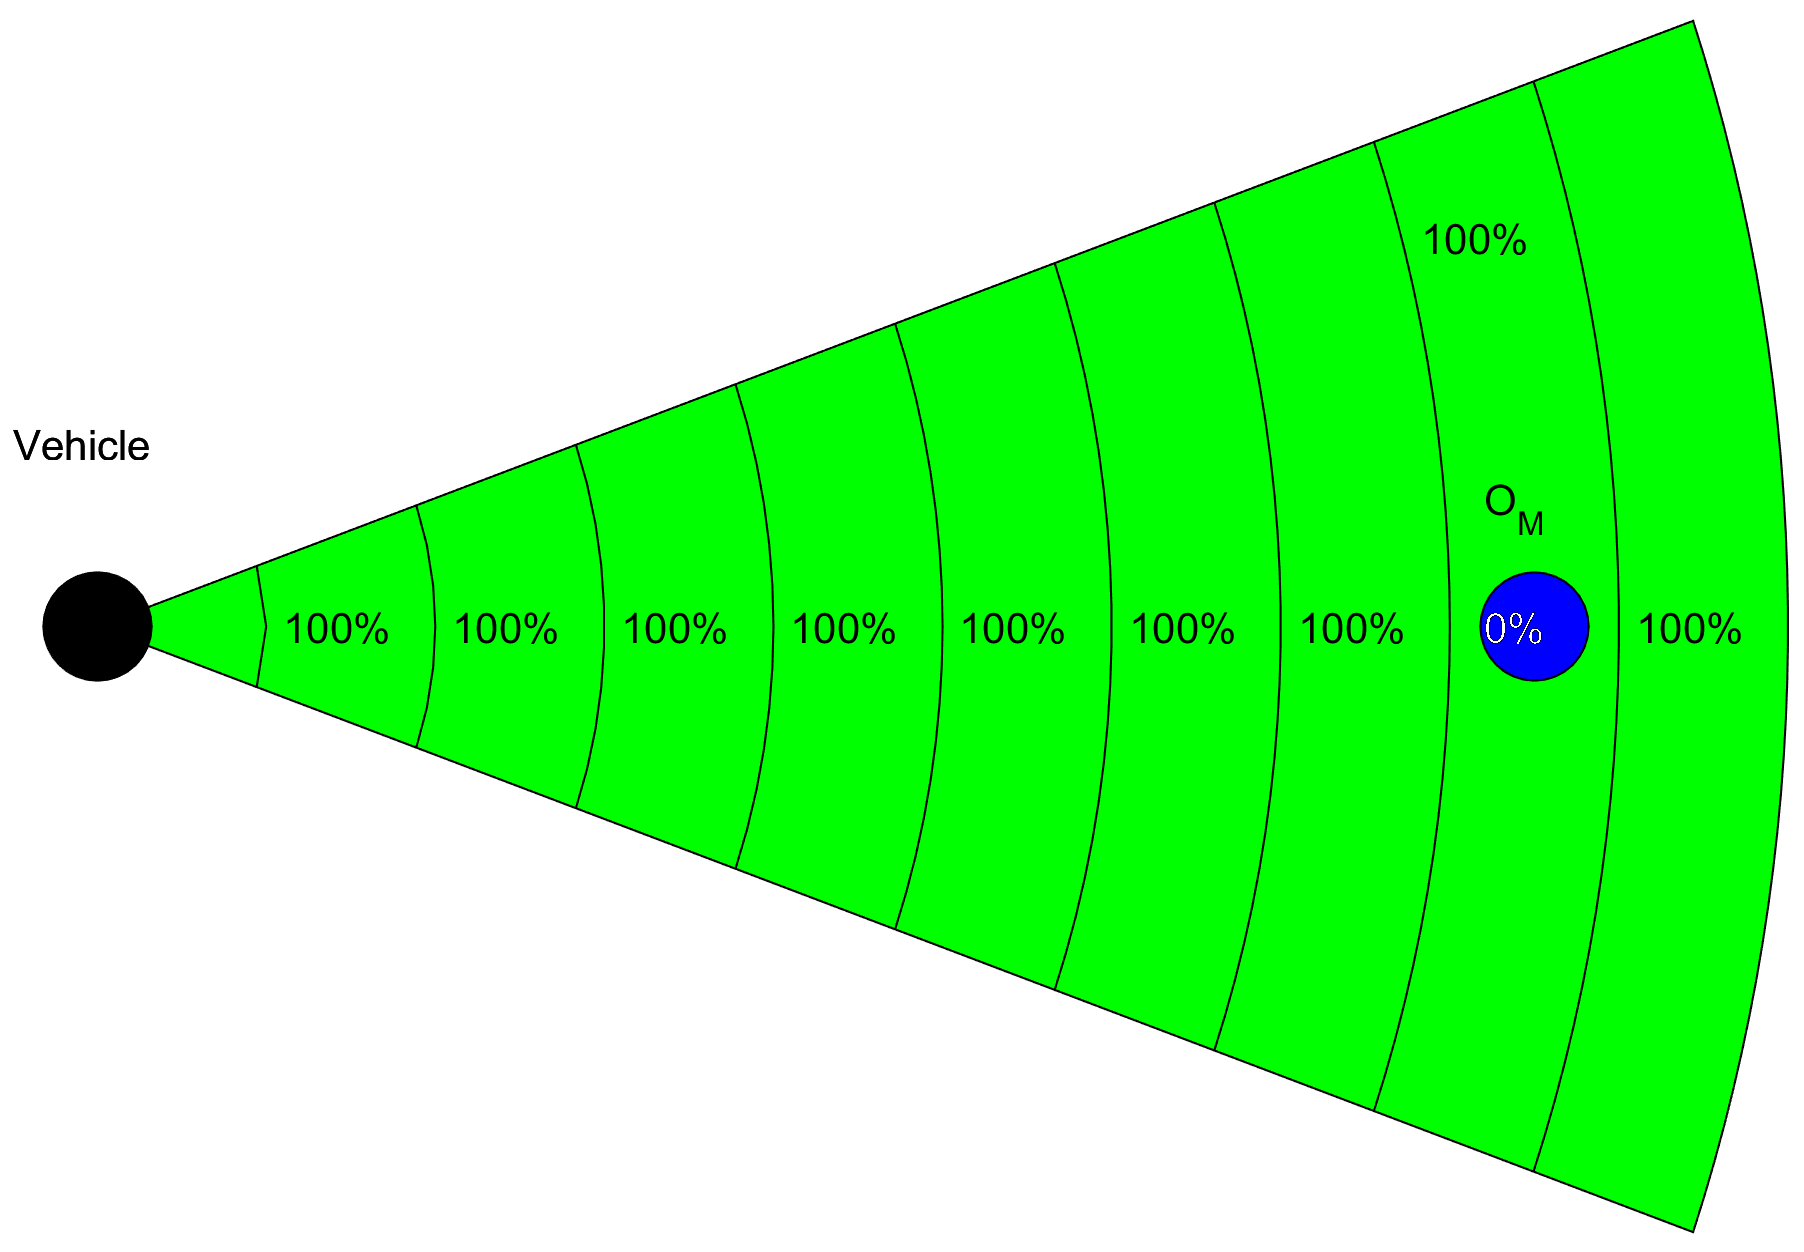
\includegraphics[width=0.9\linewidth]{\FIGDIR/TE009MapObstacleUndetected} 
            \caption{Undetected.}
            \label{fig:undetectedMapObstalce.}
        \end{subfigure}
        \begin{subfigure}{0.32\textwidth}
            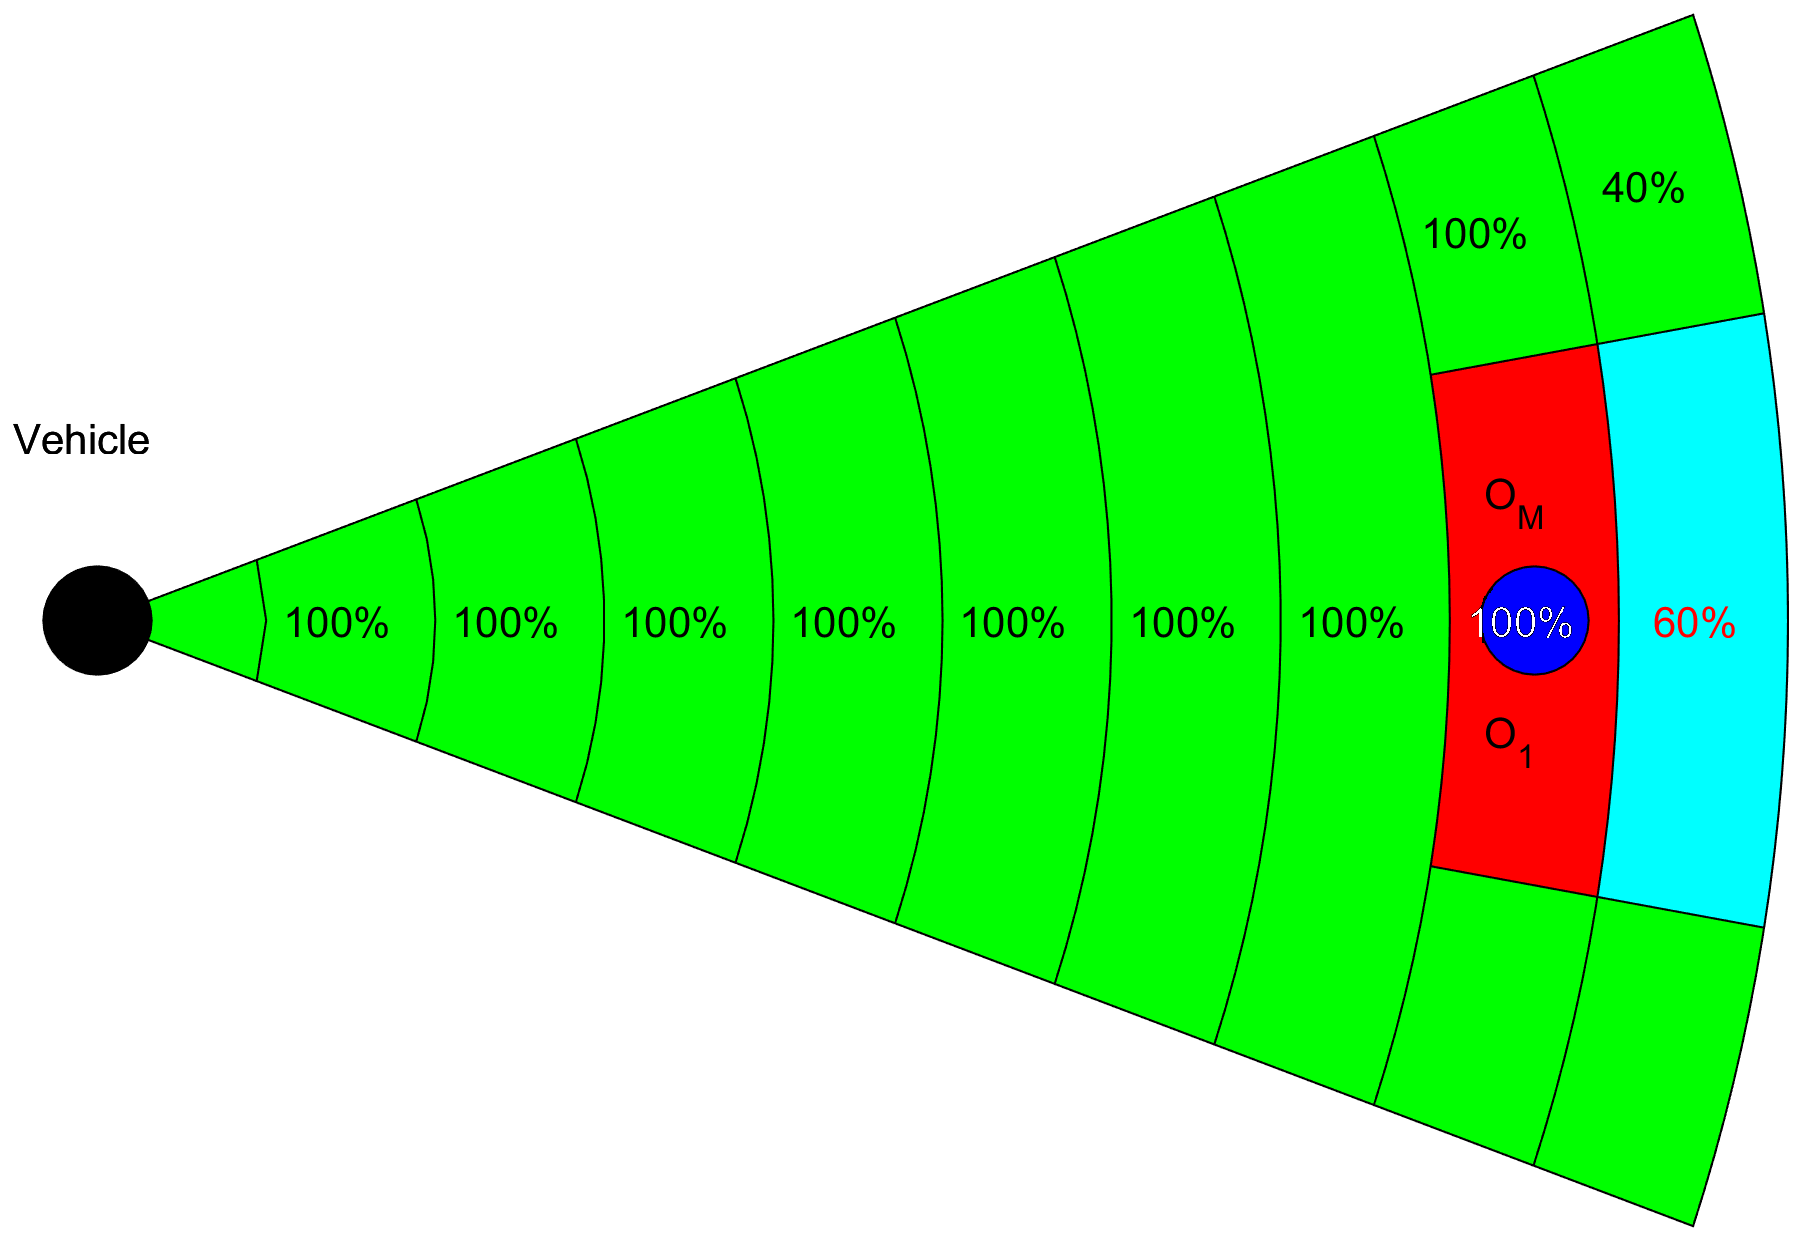
\includegraphics[width=0.9\linewidth]{\FIGDIR/TE010MapObstacleDetected} 
            \caption{Detected.}
            \label{fig:detectedMapObstacle}
        \end{subfigure}
        \begin{subfigure}{0.32\textwidth}
            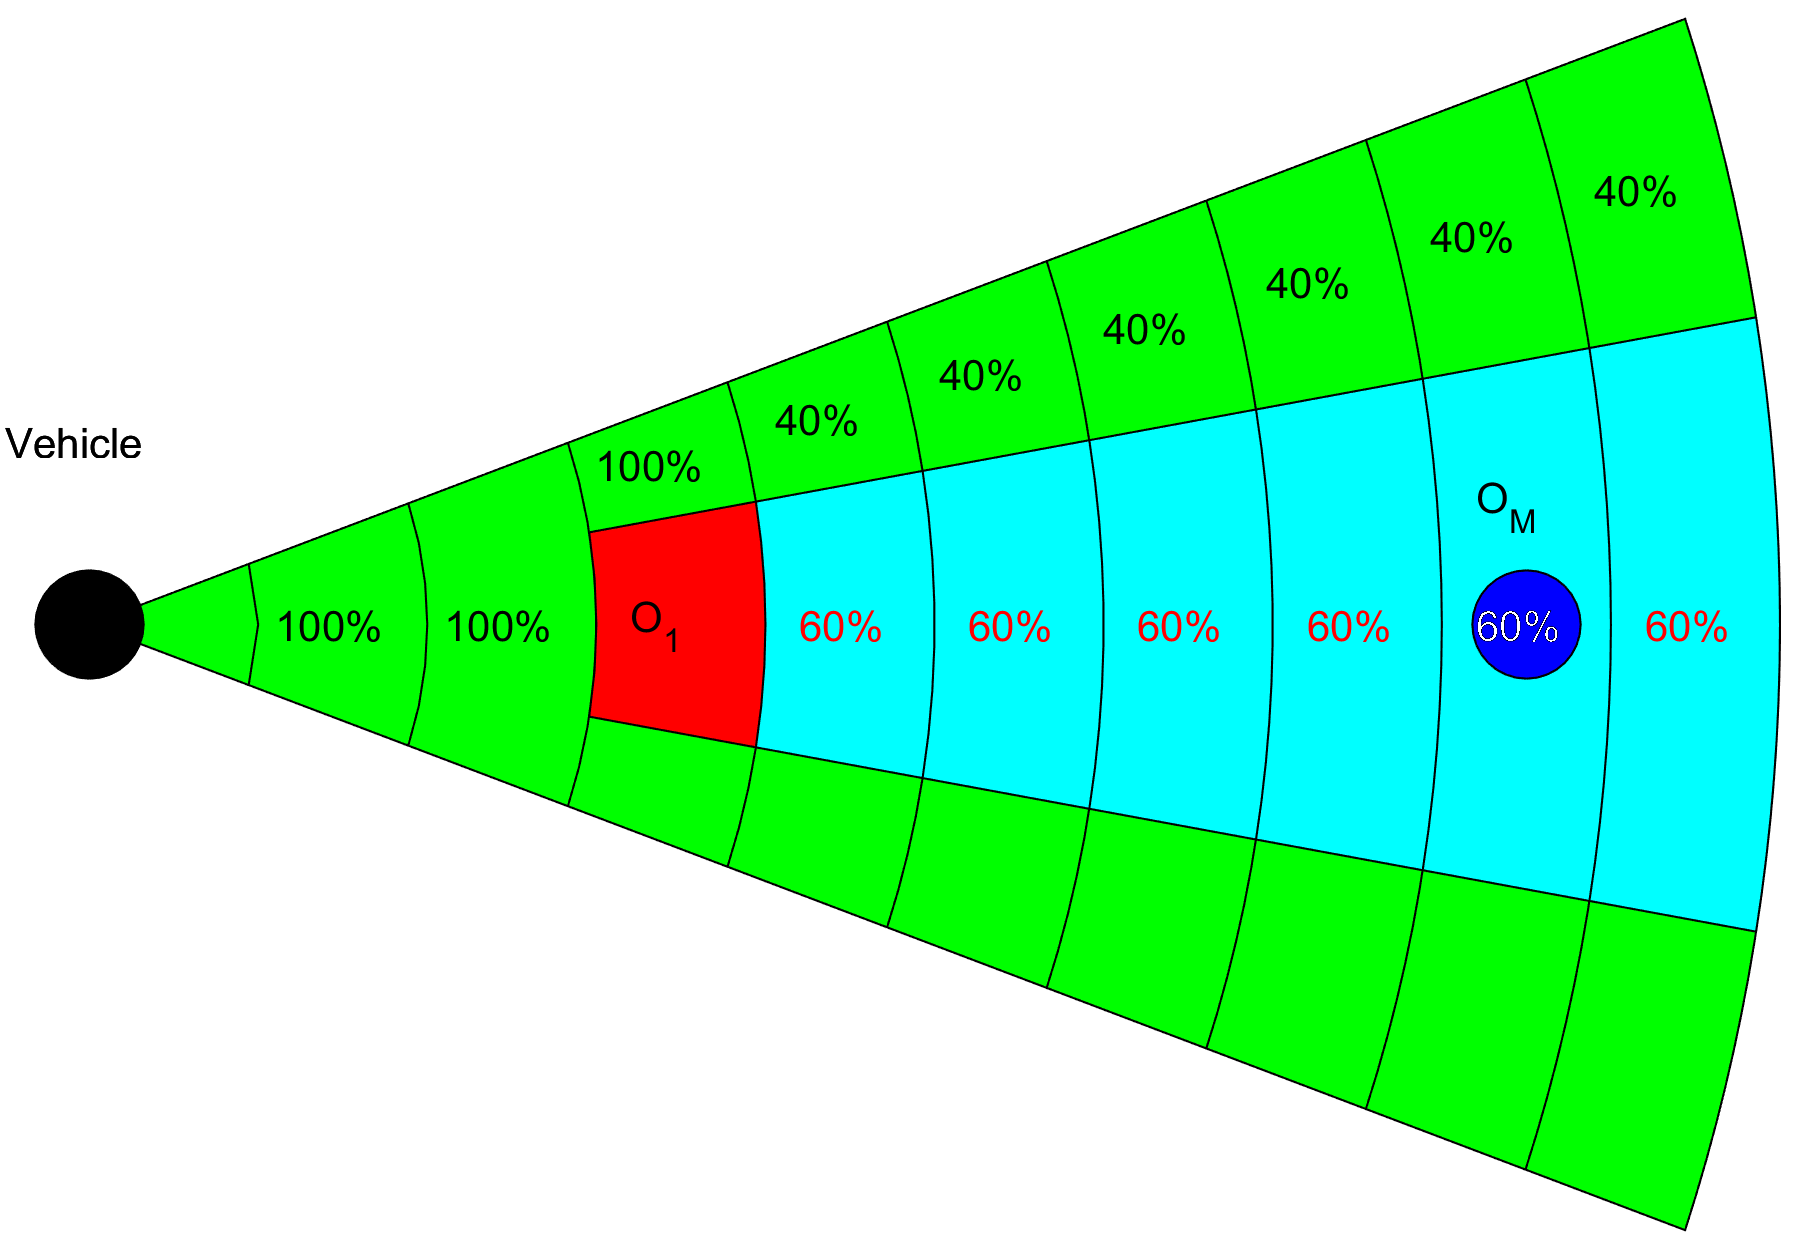
\includegraphics[width=0.9\linewidth]{\FIGDIR/TE011MapObstacleHiden}
            \caption{Hindered.}
            \label{fig:hinderedMapObstacle}
        \end{subfigure}
        \caption{Map obstacle states after \emph{Data fusion}.}
        \label{fig:mapObstacleStatesAfterDataFusion}
    \end{figure}

\subsection{(W) Virtual constraints}\label{s:virtualConstraints}
    \noindent Introduction of virtual constraints, their representation as convex polygon areas with altitude boundaries (new text)
    
